\documentclass[
11pt, % The default document font size, options: 10pt, 11pt, 12pt
%oneside, % Two side (alternating margins) for binding by default, uncomment to switch to one side
english, % ngerman for German
singlespacing, % Single line spacing, alternatives: onehalfspacing or doublespacing
%draft, % Uncomment to enable draft mode (no pictures, no links, overfull hboxes indicated)
%nolistspacing, % If the document is onehalfspacing or doublespacing, uncomment this to set spacing in lists to single
%liststotoc, % Uncomment to add the list of figures/tables/etc to the table of contents
%toctotoc, % Uncomment to add the main table of contents to the table of contents
%parskip, % Uncomment to add space between paragraphs
%nohyperref, % Uncomment to not load the hyperref package
headsepline, % Uncomment to get a line under the header
%chapterinoneline, % Uncomment to place the chapter title next to the number on one line
%consistentlayout, % Uncomment to change the layout of the declaration, abstract and acknowledgements pages to match the default layout
]{StyleSheet} % The class file specifying the document structure

\usepackage[utf8]{inputenc} % Required for inputting international characters
\usepackage[T1]{fontenc} % Output font encoding for international characters
\usepackage{palatino} % Use the Palatino font by default
\usepackage[backend=bibtex,style=authoryear,natbib=true]{biblatex} % Use the bibtex backend with the authoryear citation style (which resembles APA)
% Refer Bibliography Resource
\usepackage[autostyle=true]{csquotes} % Required to generate language-dependent quotes in the bibliography
\usepackage{graphicx}
\usepackage[space]{grffile}

\addbibresource{example.bib} % The filename of the bibliography

\geometry{
	paper=letterpaper, % Change to letterpaper for US letter
	inner=2.5cm, % Inner margin
	outer=3.8cm, % Outer margin
	bindingoffset=.5cm, % Binding offset
	top=1.5cm, % Top margin
	bottom=1.5cm, % Bottom margin
	%showframe, % Uncomment to show how the type block is set on the page
}

\thesistitle{GT Pioneer} 
% Your thesis title, this is used in the title and abstract, print it elsewhere with \ttitle

\supervisor{Dr. Raghuram \textsc{Pucha}} 
% Your supervisor's name, this is used in the title page, print it elsewhere with \supname

\examiner{} 
% Your examiner's name, this is not currently used anywhere in the template, print it elsewhere with \examname

\degree{Doctor of Philosophy} 
% Your degree name, this is used in the title page and abstract, print it elsewhere with \degreename

\author{Vishakh \textsc{Kumar}} 
% Your name, this is used in the title page and abstract, print it elsewhere with \authorname

\addresses{} 
% Your address, this is not currently used anywhere in the template, print it elsewhere with \addressname

\subject{ME 1770} 
% Your subject area, this is not currently used anywhere in the template, print it elsewhere with \subjectname

\keywords{Georgia Tech, Mars Rover, Pioneer} 
% Keywords for your thesis, this is not currently used anywhere in the template, print it elsewhere with \keywordnames

\university{\href{http://www.gatech.edu}{Georgia Institute of Technology}}

\department{\href{http://me.gatech.edu}{George W Woodruff School of Mechanical Engineering}}
% Your department's name and URL, this is used in the title page and abstract, print it elsewhere with \deptname

\group{\href{https://github.com/vishakhkumar/ME1770}{Group X}}

\faculty{\href{http://faculty.university.com}{Faculty Name}}
% Your faculty's name and URL, this is used in the title page and abstract, print it elsewhere with \facname

\AtBeginDocument{
\hypersetup{pdftitle=\ttitle} % Set the PDF's title to your title
\hypersetup{pdfauthor=\authorname} % Set the PDF's author to your name
\hypersetup{pdfkeywords=\keywordnames} % Set the PDF's keywords to your keywords
}

\begin{document}

\frontmatter % Use roman page numbering style (i, ii, iii, iv...) for the pre-content pages
\pagestyle{plain} % Default to the plain heading style until the thesis style is called for the body content

\begin{titlepage}
\begin{center}

\vspace*{.06\textheight}
{\scshape\LARGE \univname\par}\vspace{1.5cm} % University name
\textsc{\Large Project Report}\\[0.5cm] % Thesis type

\HRule \\[0.4cm] % Horizontal line
{\huge \bfseries \ttitle\par}\vspace{0.4cm} % Thesis title
\HRule \\[1.5cm] % Horizontal line

\begin{minipage}[t]{0.4\textwidth}
\begin{flushleft} \large
\emph{Author:}\\
\href{http://www.johnsmith.com}{\authorname} % Author name - remove the \href bracket to remove the link
\end{flushleft}
\end{minipage}
\begin{minipage}[t]{0.4\textwidth}
\begin{flushright} \large
\emph{Instructor:} \\
\href{http://www.me.gatech.edu/faculty/pucha}{\supname} % Supervisor name - remove the \href bracket to remove the link  
\end{flushright}
\end{minipage}\\[3cm]

\vfill

\large \textit{A report submitted in fulfillment of the requirements\\ for the team project of ME 1770}\\[0.3cm] % University requirement text
\textit{in the}\\[0.4cm]
\groupname\\\deptname\\[2cm] % Research group name and department name

\vfill

{\large \today}\\[4cm] % Date
%\includegraphics{Logo} % University/department logo - uncomment to place it

\vfill
\end{center}
\end{titlepage}

%----------------------------------------------------------------------------------------
%	ABSTRACT PAGE
%----------------------------------------------------------------------------------------

\begin{abstract}
\addchaptertocentry{\abstractname} % Add the abstract to the table of contents
The Thesis Abstract is written here (and usually kept to just this page). The page is kept centered vertically so can expand into the blank space above the title too\ldots
\end{abstract}

%----------------------------------------------------------------------------------------
%	LIST OF CONTENTS/FIGURES/TABLES PAGES
%----------------------------------------------------------------------------------------

\tableofcontents % Prints the main table of contents

\listoffigures % Prints the list of figures

\listoftables % Prints the list of tables

\mainmatter % Begin numeric (1,2,3...) page numbering
\pagestyle{thesis} % Return the page headers back to the "thesis" style

\mainmatter % Begin numeric (1,2,3...) page numbering

\pagestyle{thesis} % Return the page headers back to the "thesis" style

% Include the chapters of the thesis as separate files from the Chapters folder
% Uncomment the lines as you write the chapters

\chapter{Project Ideation}

\section{Project Proposal}
\subsection{Description of Product / Structure: Describe the creative ideation and what is new?}

Our product is a Mars capable ATV. We began with the idea of the standard ATV, coupled with the idea of a manned Mars rover. By combining these two concepts, we were able to create a more agile vehicle capable of handling Mars’ low gravity and dusty environment. The combination of a pressurized capsule in an off-road vehicle can be challenging but the benefits would be immense in creating robust vehicles for a manned colony on Mars.

\subsection{Description of subsystem}

\begin{center}
\begin{tabular}{lll}
\hline
Subsystem & Description\\
\hline
Orbital Deployment & Circular parachute and coiled spring shocks.\\
Grabbers & Pivoting arm with ball socket and grabbing hands.\\
Suspension & Coil spring shocks, double A-frame suspension and tire rods.\\
Chassis & Triangular truss support frame. \\
Tires & Cylindrical tires with embossed treads. \\
Controls & Joystick,Displays, Plexiglas encased w/ rectangular control panel.\\
Cockpit & Oblong shaped cockpit \\
Powertrain & Circular Motor with chain drive to rear axle with rear diff.\\
Charging & Rectangular solar cells on roof. \\
Science/Storage & Large prismed storage area in back of ATV. \\
Communication System & Conic Satellite Dish. \\
Lighting & Semi-Paraboloid lights mounted on front of ATV. \\
\hline
\end{tabular}
\end{center}

\subsection{Subassembly Functionality}
\begin{center}
\begin{tabular}{lll}
\hline
Subsystem & Functionality\\
\hline
Orbital Deployment & Landing Gear when ATV is dropped from orbit. \\
Grabbers & Grabs materials for data inspection.\\
Suspension & Absorbs shocks from planetary terrain. \\
Chassis & Beefy frame for surviving rough conditions.\\
Tires & Extreme grip to handle unexpected terrain. \\
Controls & Steering, cockpit, seating, etc.\\
Cockpit & Location of Controls\\
Powertrain & Electric drivetrain, differential. \\
Charging & Solar cells from roof to charge batteries behind cockpit. \\
Science/Storage & Large storage area in back of ATV to collect data/samples. \\
Communication System & Antenna to communicate with base. \\
Lighting & To maintain visibility once night falls or in sandstorms.\\
\hline
\end{tabular}
\end{center}

\subsection{Allocation for each member}

\begin{center}
\begin{tabular}{lll}
\hline
Subsystem & Member& Complexity\\
\hline
Orbital Deployment & Vishakh Kumar& Medium\\
Grabbers & Justin Sackett & Hard\\
Suspension & Asimm Hirani & Medium\\
Chassis & Juan Rodriguez & Hard\\
Tires & Auston Ferrarer& Easy\\
Controls & Vishakh Kumar & Hard\\
Cockpit & Vishakh Kumar & Easy\\
Powertrain & Asimm Hirani & Hard\\
Charging & Vishakh Kumar & Easy \\
Science/Storage & Auston Ferrarer & Medium\\
Communication System & Juan Rodriguez & Medium\\
Lighting & Justin Sackett& Easy\\
\hline
\end{tabular}
\end{center}

\subsection{Briefly explain what new functionalities (system and sub-system ) you are planning to add. How your product is different from existing products:}

This design differs from the traditional ATV because it has a improved suspension system for travel along Martian terrain. The ATV will be able to withstand orbital entry into the Martian landscape through its improved suspension and parachute for controlled descent. Additionally for increased driver visibility the pressurized cabin is built with GT-Superglass® which has the material strength of hardened steel and the weight of titanium. With this glass our vehicle will be able to withstand sandstorms containing heavy debris.

\subsection{Picture of  the Proposed System (or Similar System): (please include a reference if you are using pictures from internet). You can also include conceptual sketch.}
\begin{center}
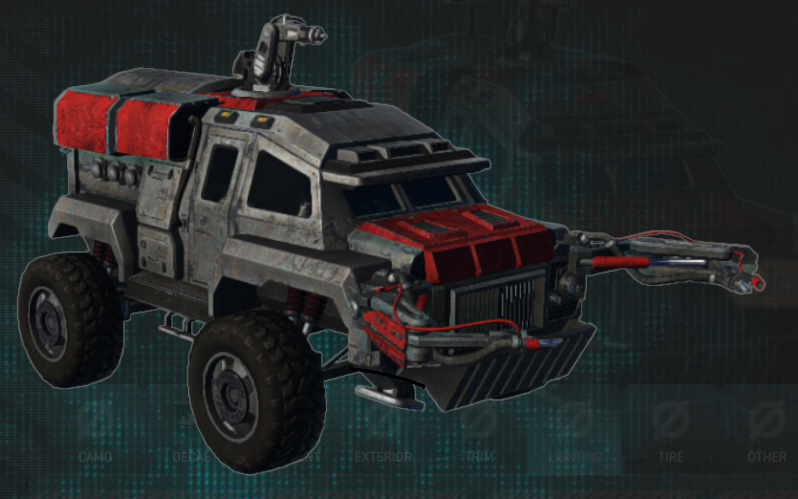
\includegraphics[width=0.75\textwidth]{a-1-1-ProjectIdeation/b-1-ProjectProposal/c-1-Images/Planetside.png} \\
(Daybreak Games: Planetside 2 ANT Vehicle Concept)

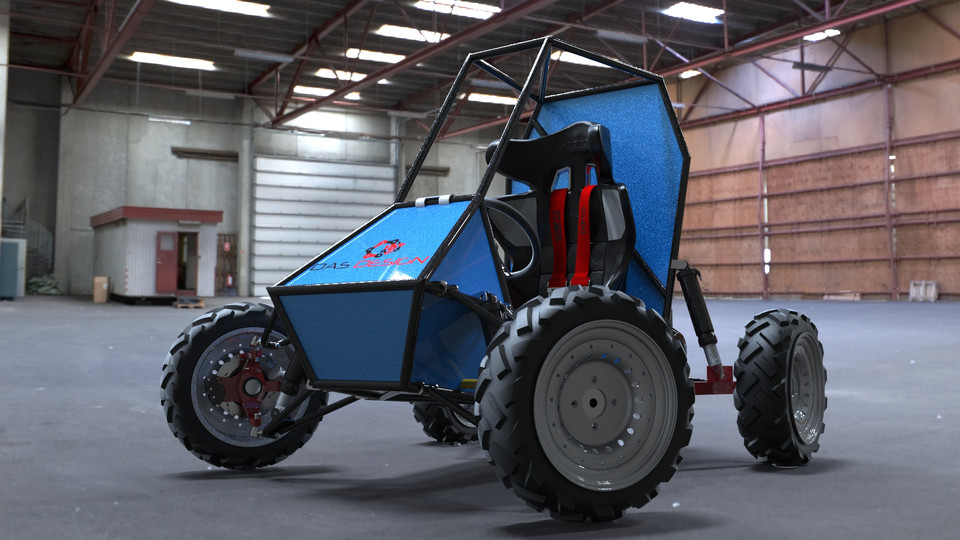
\includegraphics[width=0.75\textwidth]{a-1-1-ProjectIdeation/b-1-ProjectProposal/c-1-Images/BAJA.jpeg} \\
(https://grabcad.com/library/baja-atv-1 - BAJA SAE India Team)
\end{center}


\clearpage
 \section{Project Management}
 

Insert spiel about ProjectManagement.

\subsection{PartDistribution}
\subsubsection{Allocating subsystems among team members}

An important element of team success lies in allocating tasks to team members equitably. We kept in mind two factors while allocating tasks:

  - the set of tasks that has to be completed (which may be one task or it may be several) and
  - the set of individuals (the team members) able to complete them.

Given each team member's skill level and complexity of the part, we assigned tasks as shown in the Project Proposal (I forgot the table number).

Further description

Since the cockpit and the controls were interrelated task, it was decided to allocate both tasks to the same person.

This probably should be filled out more.


\subsection{Planning}
Insert spiel about planning.


\subsection{Timeline}
Planning our project was simple using Gantt chart created in an Excel sheet. We opted to finish our tasks earlier than suggested by the Gantt chart provided to us by our instructor due to our experience with Solidworks and inreased workload at the end of the semester from other subjects. 
We've included an image of our Gantt chart in the figure \ref{fig:GanttChart} on page \pageref{fig:GanttChart}.\\
 A detailed view of our timeline can be found at \url{https://github.com/vishakhkumar/ME1770}

\begin{figure}[!ht]
\centering
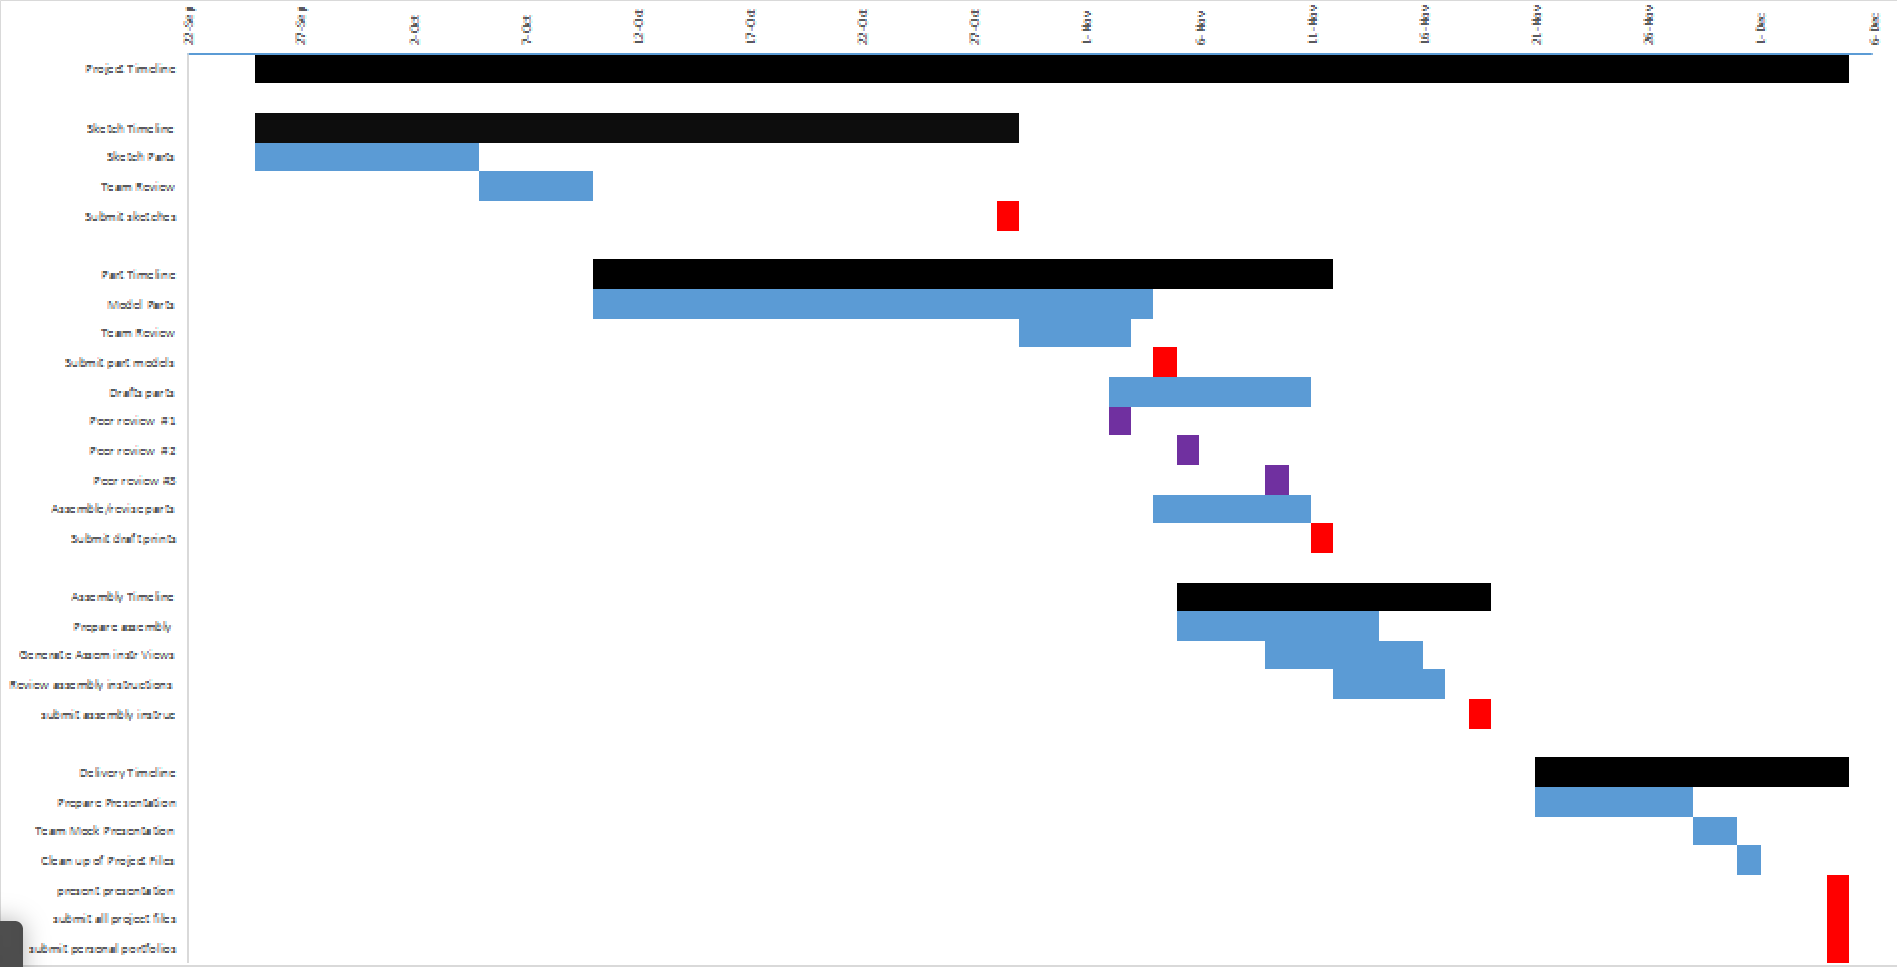
\includegraphics[angle=90,height=\textheight]{a-1-1-ProjectIdeation/b-2-ProjectManagement/Timeline.png}
\caption{Gantt Chart}
\label{fig:GanttChart}
\end{figure}



%\include{Chapters/Chapter2} 
%\include{Chapters/Chapter3}
%\include{Chapters/Chapter4} 
%\include{Chapters/Chapter5}

\end{document}
